% -*- mode:LaTex; mode:visual-line; mode:flyspell; fill-column:75-*-

\chapter{Stuff I forgot} \label{chapAppendix}

Robots are really, really great.

\section{SAM2 Box-to-Mask Tool} \label{apxSAM2}

The box-to-mask conversion of Section~\ref{secSAMAnnotation} is
performed with a purpose-built annotation tool rather than by taking
SAM2's output automatically.
For each labeled box, the tool prompts SAM2 (initialized from a base
ViT-H checkpoint, or from a fine-tuned checkpoint once one exists) with
the box and generates a set of candidate masks; the annotator steps
through these proposals and saves the one that correctly matches the
symptom, shown in Figure~\ref{figSamTool}.

\begin{figure}[h]
    \centering
    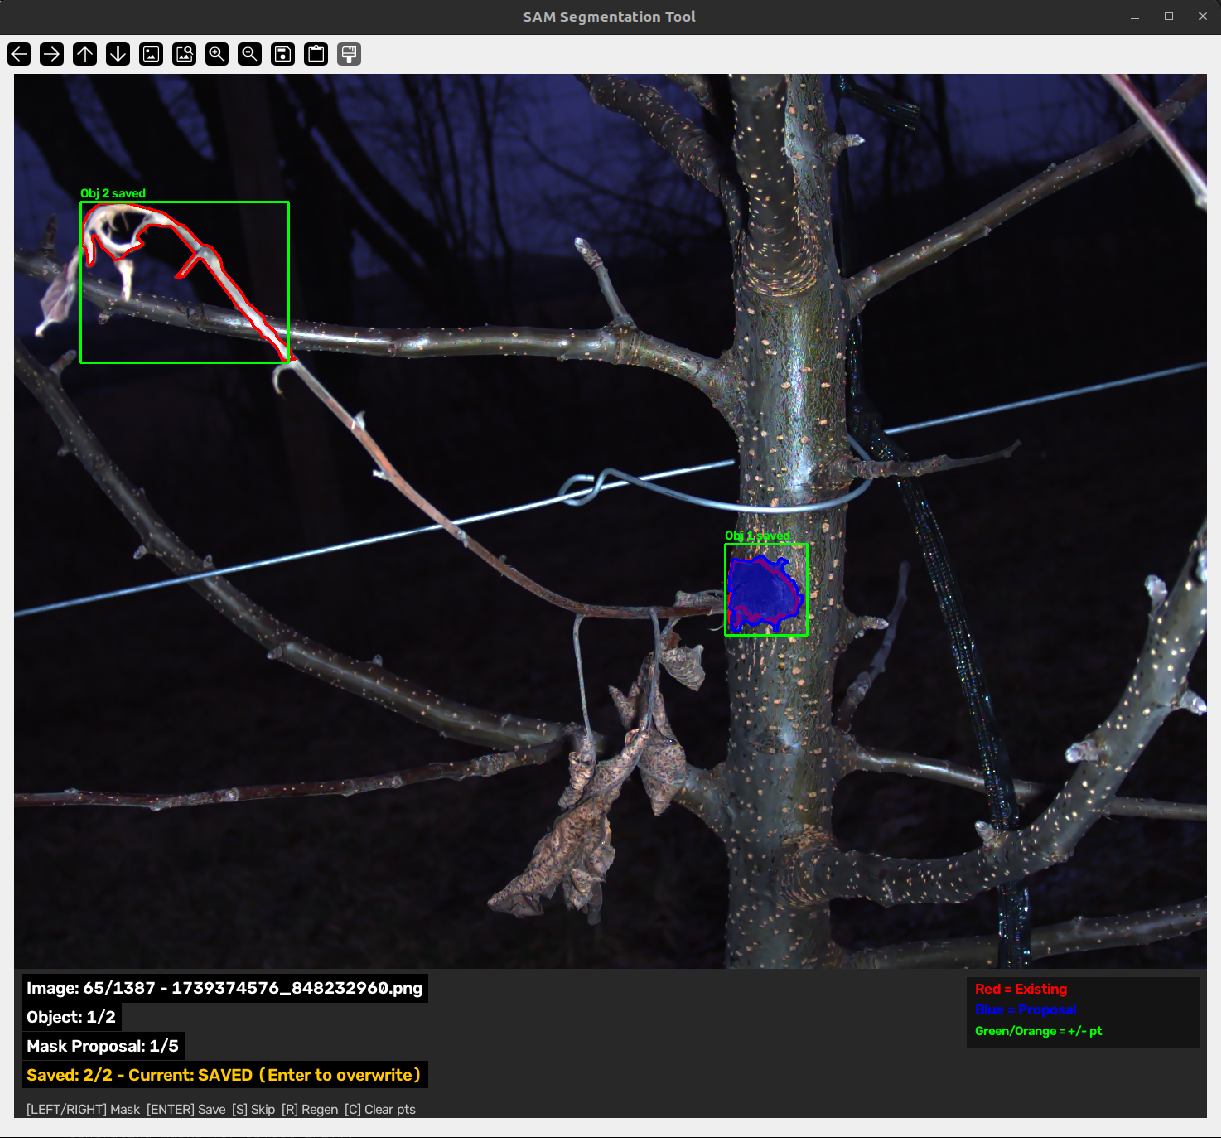
\includegraphics[width=0.8\linewidth]{figs/sam_segmentation_tool.png}
    \caption{The SAM2 box-to-mask annotation tool. The current mask
             proposal is overlaid in blue, with the existing box
             annotation outlined in red; green boxes mark objects
             already saved in the current frame. The status bar
             reports the image and object index, which of the
             candidate mask proposals is being viewed, and whether it
             has been saved, with keyboard controls to cycle proposals,
             save, skip, or regenerate.}
    \label{figSamTool}
\end{figure}

Reviewing every object by hand is the most time-consuming part of this
process, so the tool is used in two passes to reduce that cost.
An initial batch of objects is annotated interactively as described
above, and this reviewed batch is used to fine-tune SAM2's mask
decoder on the specific appearance of fire blight symptoms.
Once the fine-tuned decoder produces reliably correct top-ranked
proposals, the tool is re-run in an automatic mode that saves the
highest-confidence mask for every remaining unannotated object without
displaying it for review, leaving only objects the annotator had not
already labeled to be filled in this way.
This fine-tune-then-automate loop is what makes exhaustive mask
annotation across the full dataset practical.
